\documentclass[conference]{IEEEtran}
\IEEEoverridecommandlockouts
% The preceding line is only needed to identify funding in the first footnote. If that is unneeded, please comment it out.
\usepackage{cite}
\usepackage{amsmath,amssymb,amsfonts}
\usepackage{algorithmic}
\usepackage{graphicx}
\usepackage{textcomp}
\usepackage{xcolor}
\usepackage{subcaption}

\def\BibTeX{{\rm B\kern-.05em{\sc i\kern-.025em b}\kern-.08em
    T\kern-.1667em\lower.7ex\hbox{E}\kern-.125emX}}
\begin{document}

\title{ECE276A PR1 Report}

\author{
\IEEEauthorblockN{1\textsuperscript{st} Weixiao Zhan}
\IEEEauthorblockA{
    weixiao-zhan[at]ucsd[dot]edu}
}

\maketitle


\section{Introduction}
This report introduces a method for generating panoramic images by integrating 
a camera with an Internal Measurement Units (IMU), which includes 
accelerometer and angular velocity sensor.

In many single camera scenarios, the limited fields of view presents a challenge:
it is difficult to capture large objects within a single frame
Meanwhile, feature matching based panoramic often requires lots of computation, 
and falls short on latency sensitive applications.

To address these issues, I propose a method that utilizes IMU data to facilitate quick and 
accurate panorama image generation.
This method has broad applicability; for example, 
smartphones could utilize it to capture panoramic images, 
while robots could employ it for environmental mapping. 

The methodology involves: 1) fitting an observation model based on accelerometer data 
and a motion model based the angular velocity sensor;
2) using gradient descent to estimate a series of body rotations that 
best fit both models; 3) using the estimated rotations and 
spherical projection techniques to generate a panoramic image. 
This process could offer a more streamlined and automated solution for panoramic images.


\section{Problem Formulation}
I assume the IMU and camera are closely fixed together, 
and the combined IMU-camera unit experiences only pure rotations. 
I also neglect the translation difference between the IMU and camera frames, 
assuming the centers of the camera frame and IMU frame are aligned with the body frame.

The IMU and camera are taking samples at different interval.
Let $N^{(IMU)}$ and  $N^{(cam)} $ represent the number of samples for the IMU and camera, respectively.
Let $T^{(IMU)}_{t} $ and $T^{(cam)}_{t}$ denote the timestamp of $t$-th sample for the IMU and camera, respectively.
Define the step index $t := \left[0:N^{(IMU)}\right)$. 
The world frame is define to be aligned with body frame at time step 0.

The $t$-th IMU data includes accelerometer $a_t \in \mathbb{R}^3$ and 
angular velocity $ w_t \in \mathbb{R}^3$, both in body frame.
I use a quaternion $q_t \in H_*$ to represent the rotation from body to
world fame at timestamp $T^{(IMU)}_{t} $.
The interval between each time step can be calculated as: 
$$\tau = T^{(IMU)}_{[1:]} - T^{(IMU)}_{[:-1]}$$


\subsection{Motion and Observation Model}

The motion model infers the next rotation from current rotation and angular velocity.
Formally:
$$q_{t+1} \sim f(q_t, \tau_t, w_t) = q_t \circ \exp([0, \tau_t w_t/2])$$

The observation model infers current rotation from current gravity acceleration.
Formally:
$$a_t \sim h(q_t) = q_t^{-1} \circ [0, a_0] \circ q_t$$
In which, $a_0$ is the gravity acceleration at time step 0. By definition, 
this is also the gravity acceleration in world frame.

\subsection{Loss Function}

Our best best estimate rotations should fits in both the motion and observation model.
Formally:
$$
\begin{aligned}
    \text{mloss} =&\sum^{N^{(IMU)}-2}_{t=0} \| 2\log \left( q^{-1}_{t+1}\circ f\left( q_{t},\tau_{t} ,w_{t}\right)  \right)  \|^{2}_{2} \\ 
    \text{oloss} =&\sum^{N^{(IMU)}-1}_{t=1} \| a_{t}-h(q_{t})\|^{2}_{2} \\ 
    \text{best estimate} =&\arg \min_{\forall q} \left( \lambda \text{mloss} + (1-\lambda)\text{oloss} \right)  
\end{aligned} 
$$
In which, I introduced preference coefficient $\lambda$ to adjust how much the estimation
should favor motion model or observation model.

\subsection{Panorama}
After obtained estimated rotations, I project images to a sphere (illustrates in Figure \ref*{fig:FOV}), apply rotations, 
and finally project to a cylinder image (illustrates in Figure \ref*{fig:cylinder}).

\begin{figure}[h]
    \centering
    \begin{subfigure}{0.2\textwidth}
        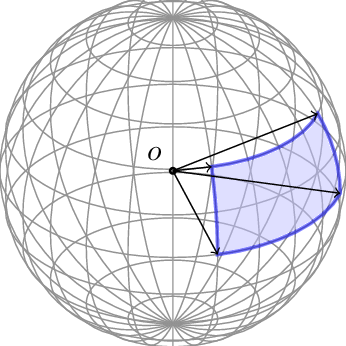
\includegraphics[width=\linewidth]{fov.png}
        \caption{FOV projection}
        \label{fig:FOV}
    \end{subfigure}
    \hfil
    \begin{subfigure}{0.2\textwidth}
        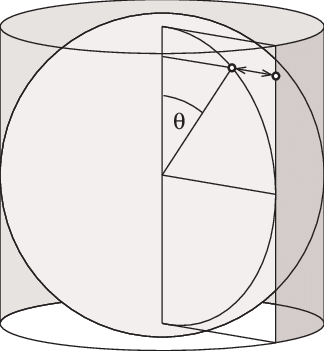
\includegraphics[width=\linewidth]{area-preserving-mapping-of-a-sphere-onto-a-cylinder.png}
        \caption{cylinder projection}
        \label{fig:cylinder}
    \end{subfigure}
    \caption{Projections}
\end{figure}

Let the camera image has $\left(\text{imglen}_{x} \times \text{imglen}_{y}\right)$ pixels
and $\left(\text{imgfov}_{x} \times \text{imgfov}_{y}\right)$ radian field of view.
Thus, the radius of intermediate sphere 
$r := \frac{\text{imglen}}{\text{imgfov}}$ pixels,
the hight of cylinder is $2r$, 
and the length of cylinder is the circumference of sphere $2\pi r$.
Let $\left(\text{img}^{(t)}_{x}, \text{img}^{(t)}_{y}\right)$ 
denote one pixel's coordinate on raw image, 
and $\left(\text{cylinder}_{x}, \text{cylinder}_{y}\right)$
denote that pixel projection's coordinate on cylinder image.


\begin{enumerate}
    \item Pixel's coordinate on raw image are 
    mapped to spherical coordinates with radius $r$, 
    then converted to Cartesian coordinates.
    $$
    \begin{aligned}
    \left[ \begin{matrix}\phi \\\theta \end{matrix} \right]  
        &=\left[ \begin{matrix}
            \text{imgfov}_{x} (\frac{1}{2} -\frac{\text{img}^{(t)}_{x}}{\text{imglen}_{x}} ) \\
            \text{imgfov}_{y} (\frac{1}{2} -\frac{\text{img}^{(t)}_{y}}{\text{imglen}_{y}} )
        \end{matrix} \right]  \\
    \left[ \begin{matrix}x\\y\\z\end{matrix} \right]_c  
        &=r\left[ \begin{matrix}
            \cos \theta \cos \phi \\
            \cos \theta \sin \phi \\
            \sin \theta 
        \end{matrix} \right]  
    \end{aligned} 
    $$

    \item Each image is associated with the estimated rotation with 
    closest-in-the-past timestamp $q_t$ and the ground truth rotation matrix $R_t$. 
    Apply the associated rotations to Cartesian coordinates.
    $$
    \begin{aligned}
        \left[ \begin{matrix}0&x&y&z\end{matrix} \right]_{r}  =&q_{t}\circ \left[ \begin{matrix}0&x&y&z\end{matrix} \right]_{c}  \circ q^{-1}_{t}\\ 
        \left[ \begin{matrix}x\\y\\z\end{matrix} \right]_{r}  =&R_{t}\left[ \begin{matrix}x\\ y\\ z\end{matrix} \right]_{c}  
    \end{aligned} 
    $$

    \item Use an area-preserving mapping, shown in Figure \ref*{fig:cylinder}, from sphere onto a cylinder.
    $$
    \left[ \begin{gathered}\text{cylinder}_{x} \\ \text{cylinder}_{y} \end{gathered} \right]  =\left[ \begin{matrix}\left( \pi -\arctan \left( y_{r},x_{r}\right)  \right)  r\\ r-z_{r}\end{matrix} \right]  
    $$

    \item With coordinate mapping, set the pixel on cylinder to RGB value of the pixel on original image.
    $$
    \text{cylinder}\left[\text{cylinder}_{x}, \text{cylinder}_{y}\right] \leftarrow 
    \text{img}^{(t)}\left[\text{img}_{x}, \text{img}_{y}\right]
    $$

\end{enumerate}


\section{Technical Approach}
\subsection{Data preprocessing}
Following the guidelines in the IMU reference, 
I converted the raw data to physical units. 
I observed that the bias in angular velocity significantly varies across the three axes. 
Assigning a unique bias to each axis substantially reduced the error in the motion model. 
However, the accelerometer did not exhibit such a bias variance across its three axes.

\subsection{Initial values}
I employed two methods of generating my initial values.
The first method involves using motion model and intergrade over time. 
The second method relies on observation models.
I utilized the cross product of $a_t$ and $a_0$ to obtained 
axis-angle representation of rotation from body frame to world frame, 
which I then convert it to quaternion.
The results indicate that initial values derived from the observation model sometimes 
resulted in better outcomes, 
with smaller loss compared to those obtained from the motion model and random initial values. 
However, this advantage diminishes if the body experiences not only pure rotation 
but also some acceleration, 
making the observation model less reliable due to inertial forces.

\subsection{Gradient descent}
I used NumPy and Pytorch(CPU) to manage in-memory data and accelerate computation;
I implemented quaternion exp and log
\footnote{quaternion norms are added 1e-12 to prevent divide-by-zero}
, motion model $f$, observation model $h$ and loss function in PyTorch to allow auto-gradient.
Additionally, an early-stop mechanism is incorporated into the training loop.

The preference coefficient $\lambda$ is set to $\frac12$,
learning rate to 1e-3,
training epoch to 6000,
and early stop patient to 10.
In most trainings, the early-stop breaks the training loop before epoch running out .

\subsection{Projections}
$$\text{imglen}_{x} = 320, \text{imglen}_{y}=240$$
$$\text{imgfov}_{x} = \frac{\pi}{6}, \text{imgfov}_{y} = \frac{\pi}{8}$$

The radius $r$ is round to 306 and the circumference is round to 1923.

\section{Results}
Data set 1,2,8,9,10,11,3,4,5,6,7 are present in Figure
\ref*{fig:set1} to \ref*{fig:set7}.
The average loss on train set is $6.561$, 
and average loss on test set is $7.946$.

Sub-figure a(s) are the quaternion representation of the rotations.
Sub-figure b(s) are the Euler angles representation of the rotation.
In Sub-figure a(s) and b(s), the solid blue line shows the gradient descent results;
the orange and green dot lints show the motion and observation model's initial values; 
the red dash line shows the ground truth.
Sub-figure c(s) show the panorama image based on gradient descent rotations;
sub-figure d(s) show the panorama image based on ground truth rotations.
Full size images can be find at \texttt{img/} directory.

Findings
\begin{enumerate}
\item In must dataset, the gradient descent results followed the ground truth.
The projection successfully assembles images into coherent panoramic views of the environment.

\item Quaternion $q$ and $-q$ are representing the same rotation, 
Therefore, in certain sections, such as sub-figure \ref*{fig:8qt} and \ref*{fig:9qt},
the gradient descent results and ground truth appear flipped on the diagram,
despite representing proximate rotations.

\item Euler angles exhibit singularities, causing oscillations in the plots, 
as observed in sub-figure \ref*{fig:1ea}. 
This makes Euler angles difficult to interpret in those cases.

\item In some datasets, the discrepancy between motion model and observation models 
is minor. However, in others, such as data set 9, 10 and 11, 
observation model significantly deviates from both the motion model and the ground truth.
This deviation could be attributed to 360-degree rotations performed by the body, 
during which the linear accelerations become significant and breaks the pure rotation assumption.

\item The last approximately 20\% of the camera images in data set 1, 2 have
translations, specifically, a vertical downward movement.
This contradicts the foundational assumption of purely rotational body frame movement. 
Consequently, these images were manually excluded from panorama stitching.

\item A model incorporating the translational differences between the camera and IMU 
might further enhance the quality of the generated panoramas.

\item Utilizing the angular velocity sensor for rotation estimation and 
the accelerometer for velocity estimation could potentially allow for 
a comprehensive full body poses estimation, 
offering a more accurate model of camera movement.

\end{enumerate}

Overall, the estimated rotation allows realistic panorama generation.
The in-perfection could be largely caused by non-pure rotation 
and numerical errors.
The most challenging part of the project is to calibrate the 
IMU data, finding out their correct signs and bias.

\begin{figure}[h]
    \centering
    \begin{subfigure}{0.4\textwidth}
        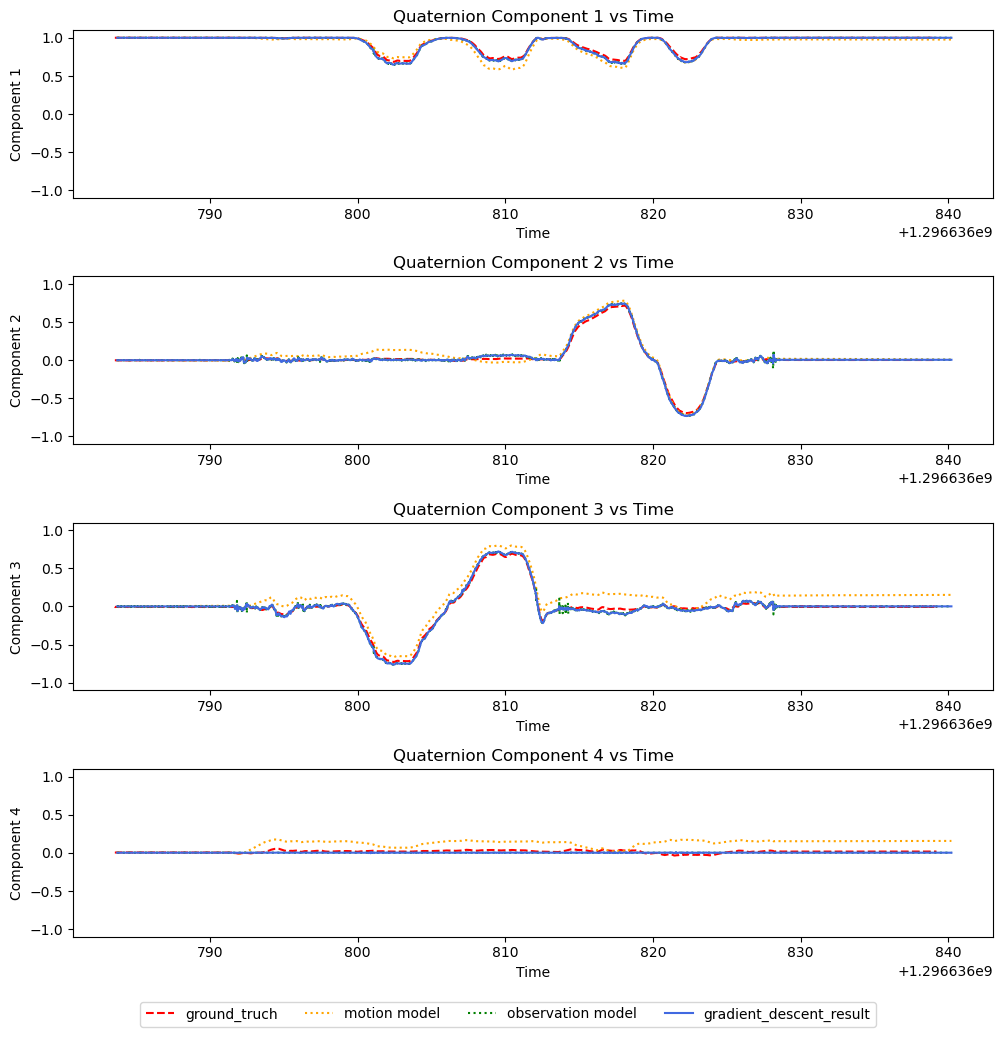
\includegraphics[width=\linewidth]{../img/1_qt.png}
        \caption{quaternion}
        \label{fig:1qt}
    \end{subfigure}
    \hfill
    \begin{subfigure}{0.4\textwidth}
        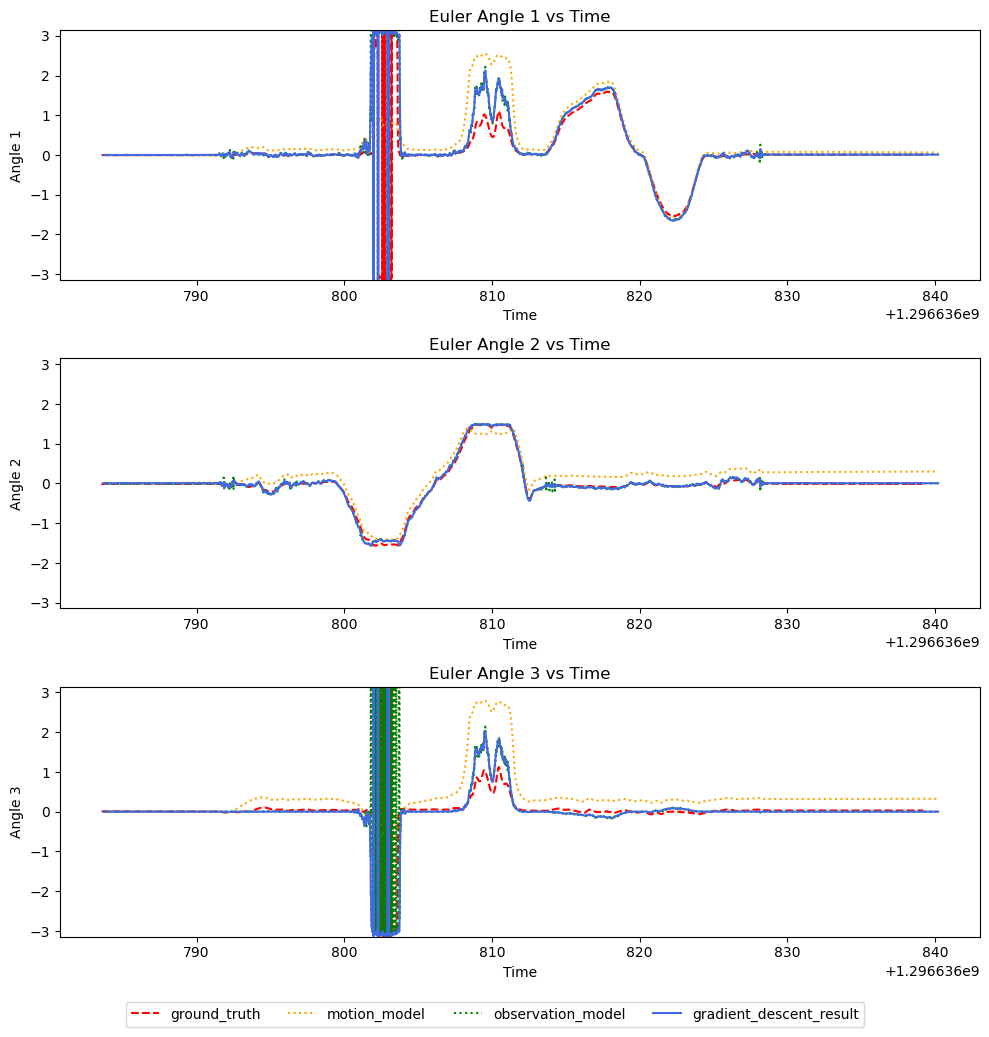
\includegraphics[width=\linewidth]{../img/1_ea.png}
        \caption{Euler angles}
        \label{fig:1ea}
    \end{subfigure}
    \begin{subfigure}{0.4\textwidth}
        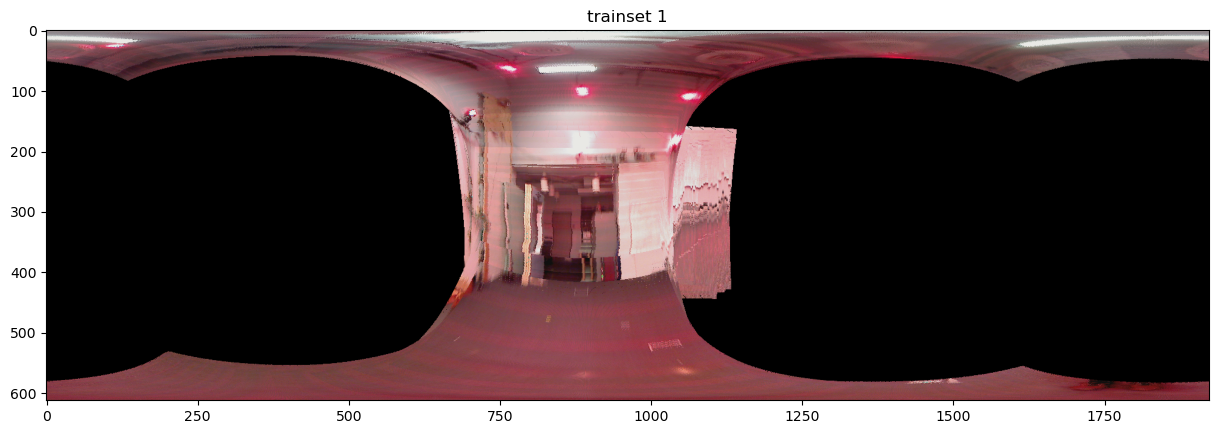
\includegraphics[width=\linewidth]{../img/pano_1_gd.png}
        \caption{gradient descent results}
        \label{fig:1p}
    \end{subfigure}
    \begin{subfigure}{0.4\textwidth}
        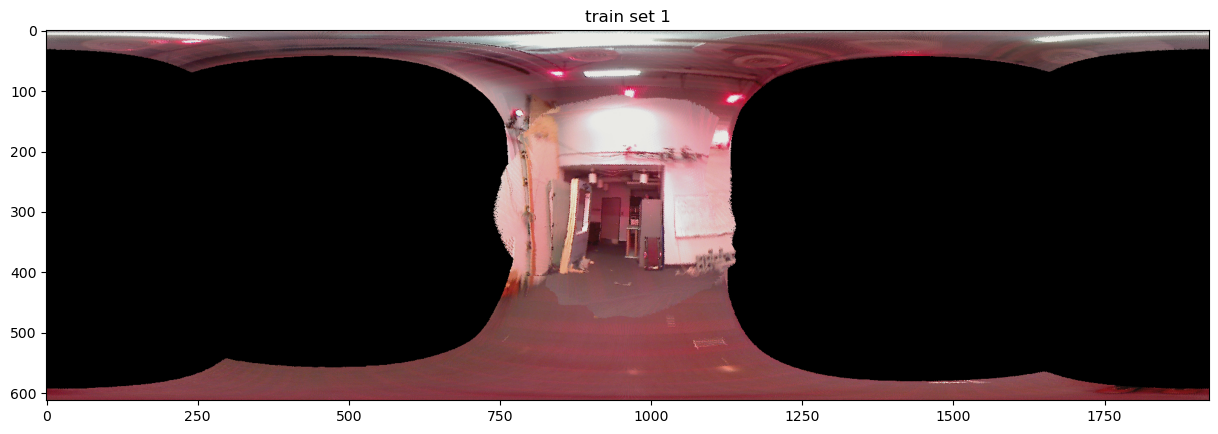
\includegraphics[width=\linewidth]{../img/pano_1_gt.png}
        \caption{ground truth results}
        \label{fig:1pt}
    \end{subfigure}

    \caption{Train set 1}
    \label{fig:set1}
\end{figure}

\begin{figure}[h]
    \centering
    \begin{subfigure}{0.4\textwidth}
        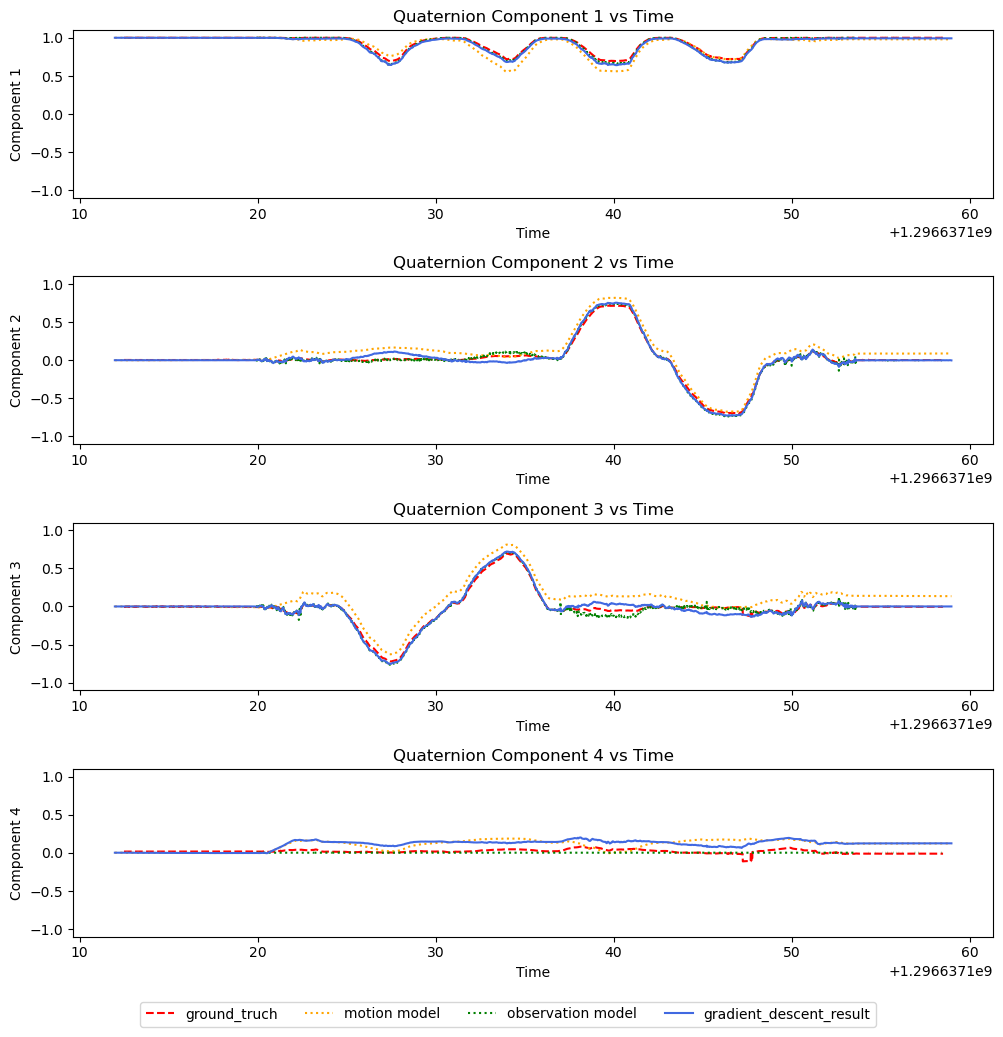
\includegraphics[width=\linewidth]{../img/2_qt.png}
        \caption{quaternion}
        \label{fig:2qt}
    \end{subfigure}
    \hfill
    \begin{subfigure}{0.4\textwidth}
        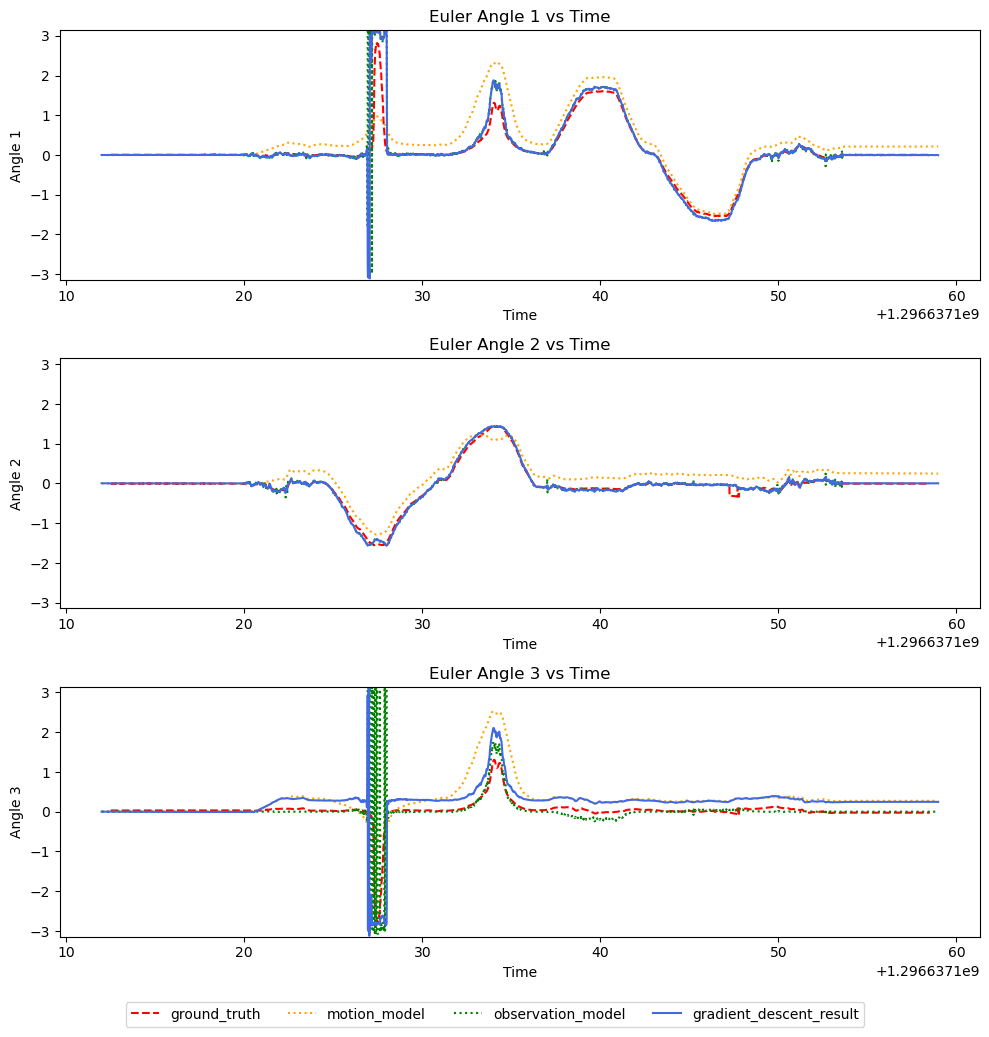
\includegraphics[width=\linewidth]{../img/2_ea.png}
        \caption{Euler angles}
        \label{fig:2ea}
    \end{subfigure}
    \begin{subfigure}{0.4\textwidth}
        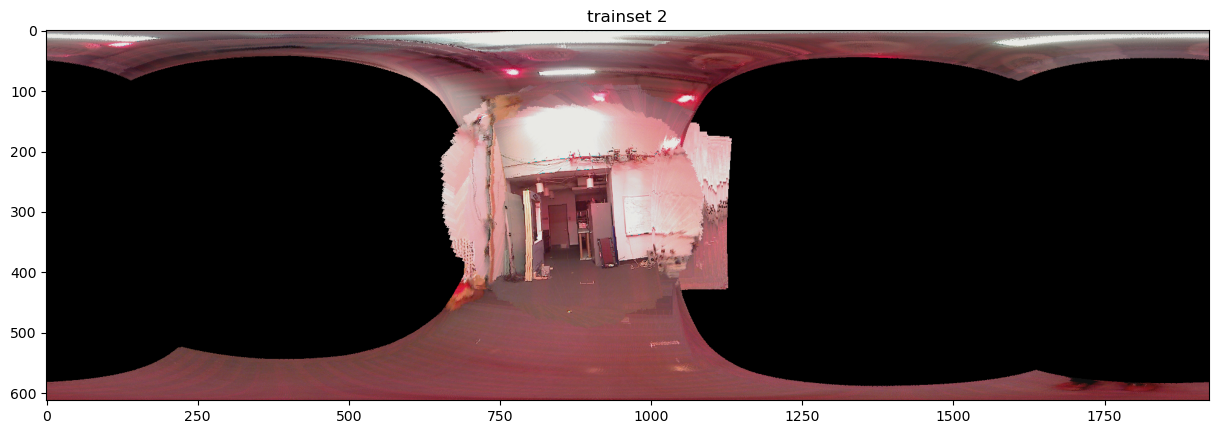
\includegraphics[width=\linewidth]{../img/pano_2_gd.png}
        \caption{gradient descent results}
        \label{fig:2p}
    \end{subfigure}
    \begin{subfigure}{0.4\textwidth}
        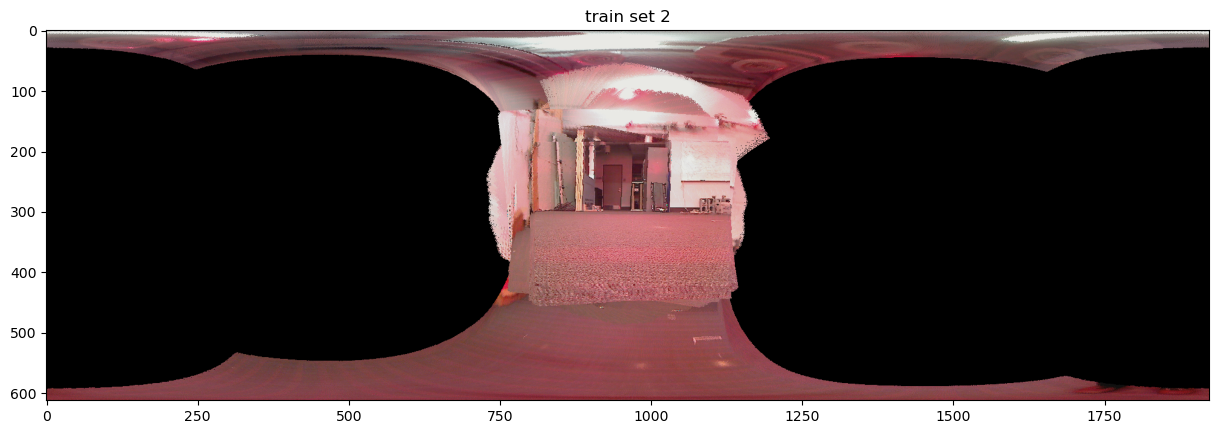
\includegraphics[width=\linewidth]{../img/pano_2_gt.png}
        \caption{ground truth results}
        \label{fig:2pt}
    \end{subfigure}

    \caption{Train set 2}
    \label{fig:set2}
\end{figure}

\begin{figure}[h]
    \centering
    \begin{subfigure}{0.4\textwidth}
        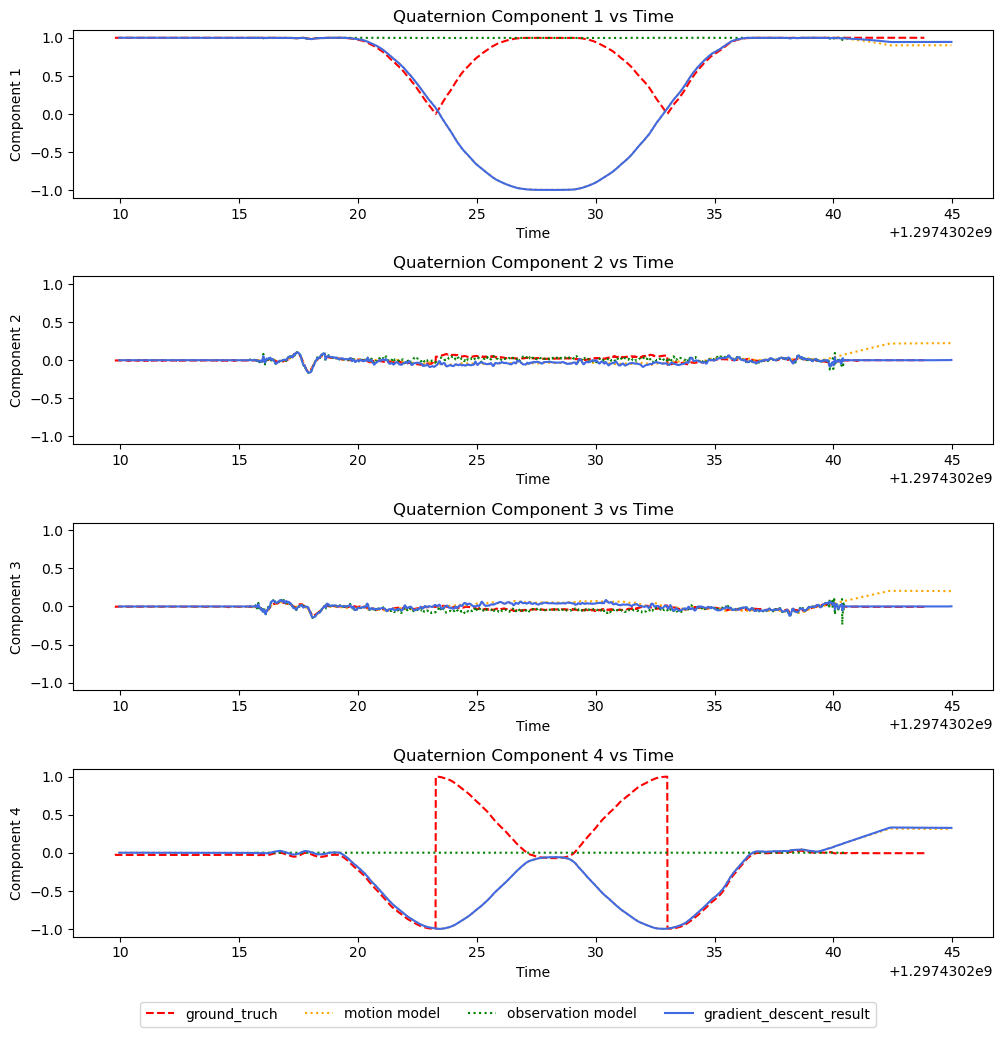
\includegraphics[width=\linewidth]{../img/8_qt.png}
        \caption{quaternion}
        \label{fig:8qt}
    \end{subfigure}
    \hfill
    \begin{subfigure}{0.4\textwidth}
        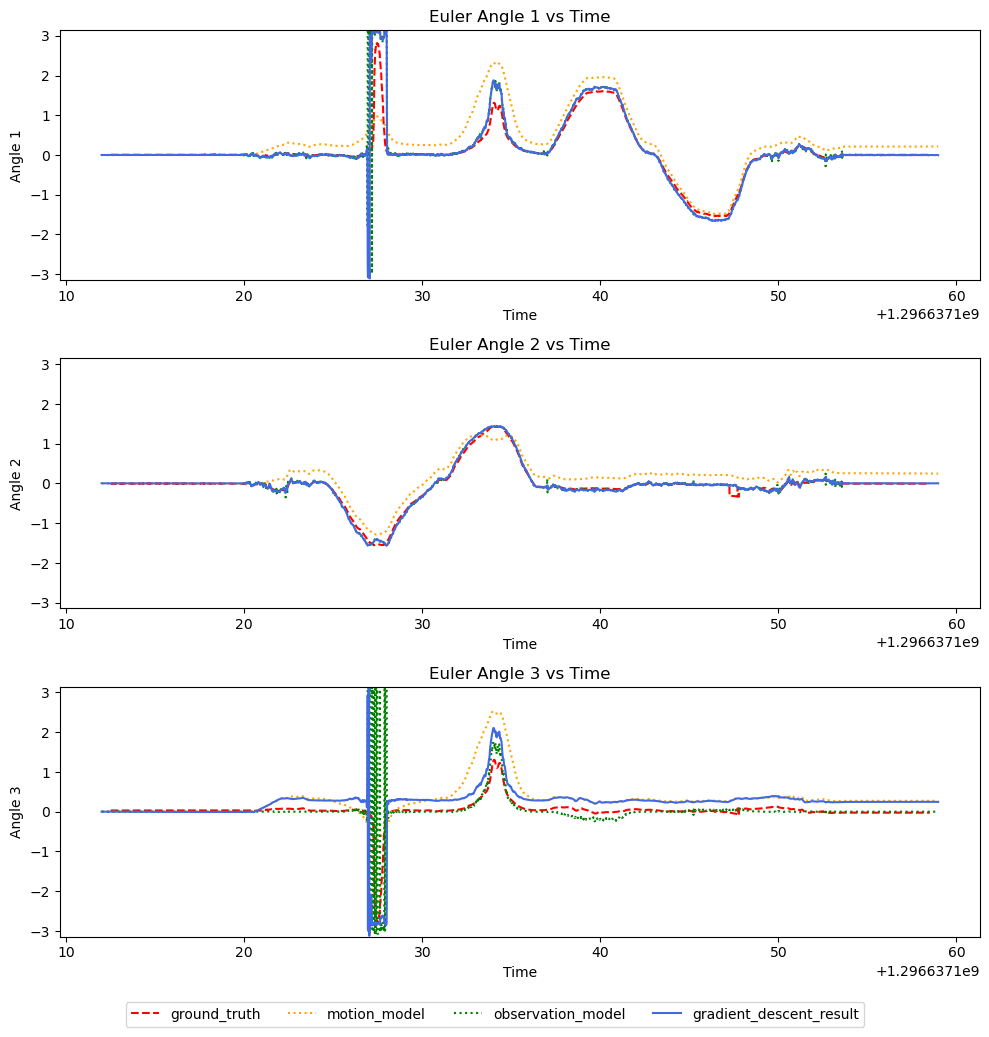
\includegraphics[width=\linewidth]{../img/2_ea.png}
        \caption{Euler angles}
        \label{fig:8ea}
    \end{subfigure}
    \begin{subfigure}{0.4\textwidth}
        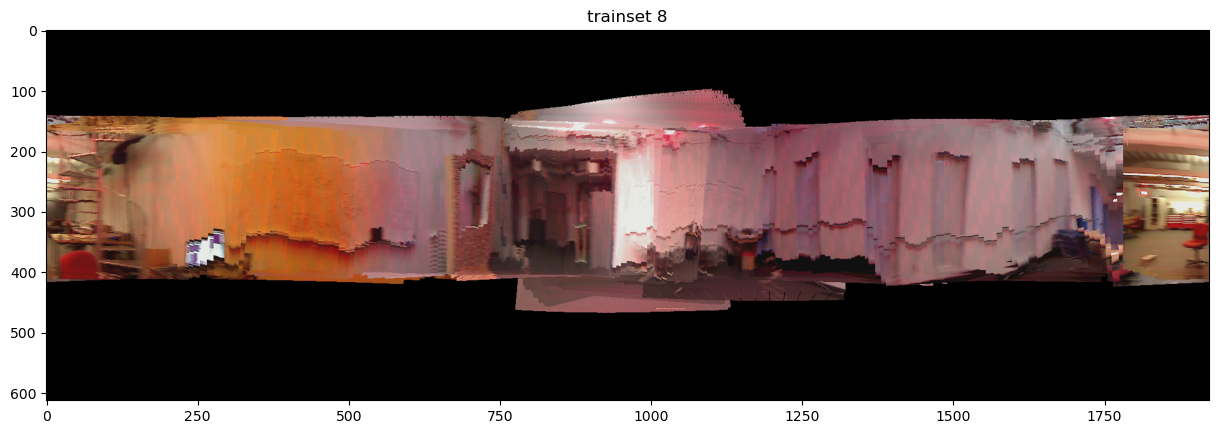
\includegraphics[width=\linewidth]{../img/pano_8_gd.png}
        \caption{gradient descent results}
        \label{fig:8p}
    \end{subfigure}
    \begin{subfigure}{0.4\textwidth}
        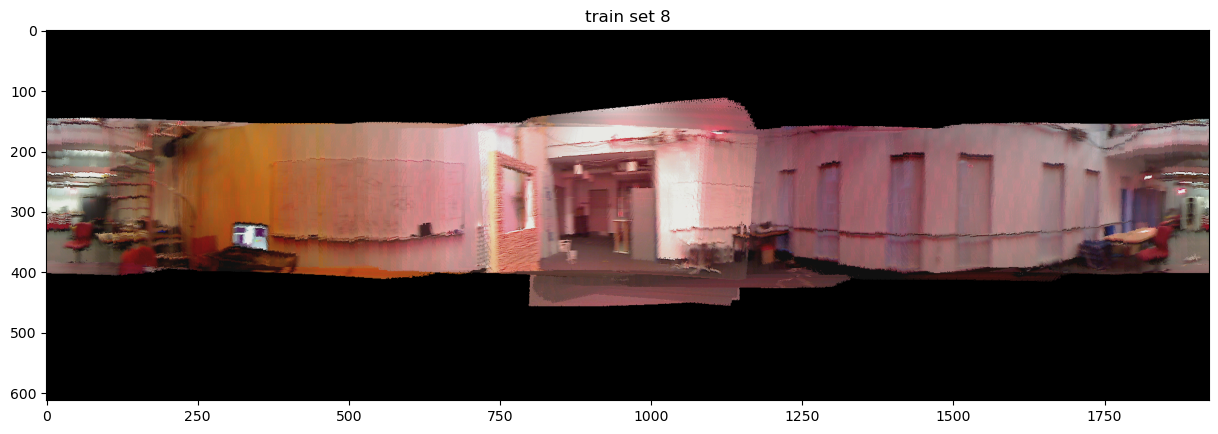
\includegraphics[width=\linewidth]{../img/pano_8_gt.png}
        \caption{ground truth results}
        \label{fig:8pt}
    \end{subfigure}

    \caption{Train set 8}
    \label{fig:set8}
\end{figure}

\begin{figure}[h]
    \centering
    \begin{subfigure}{0.4\textwidth}
        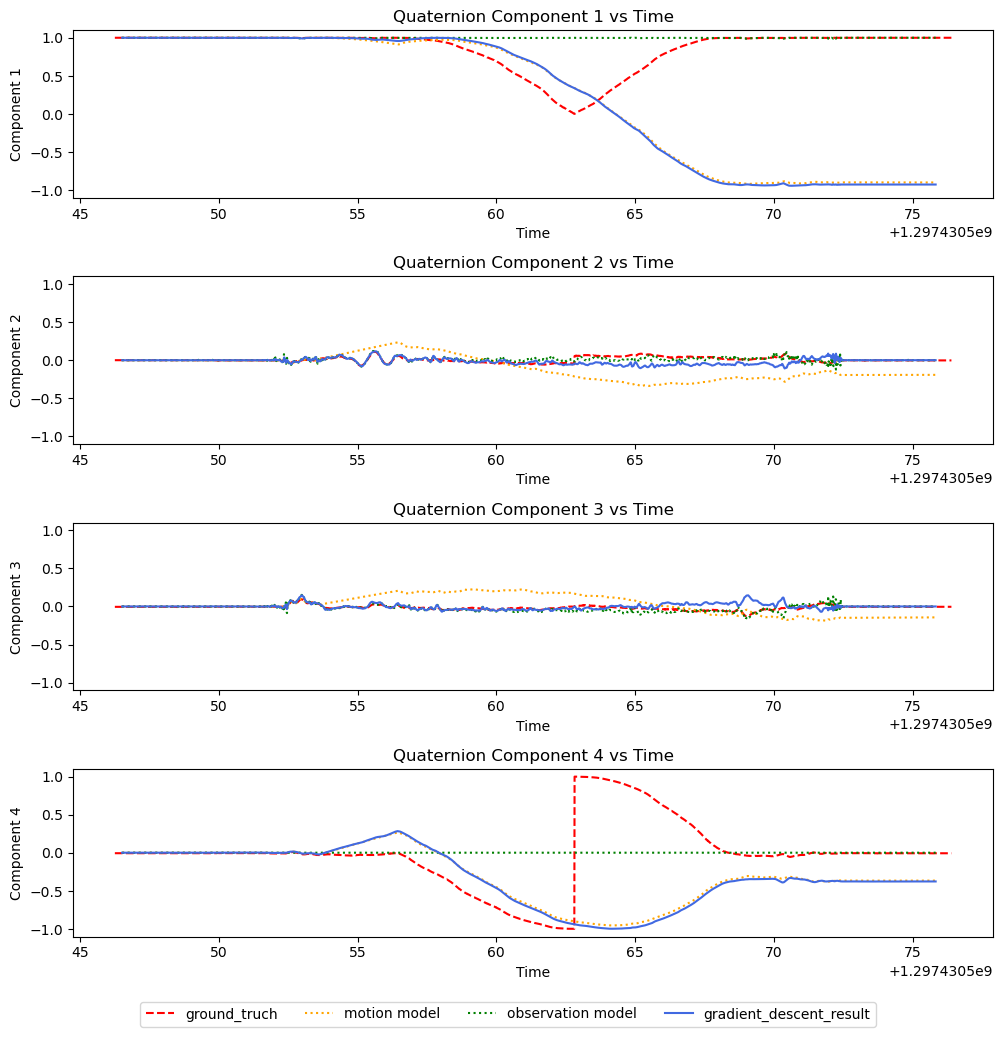
\includegraphics[width=\linewidth]{../img/9_qt.png}
        \caption{quaternion}
        \label{fig:9qt}
    \end{subfigure}
    \hfill
    \begin{subfigure}{0.4\textwidth}
        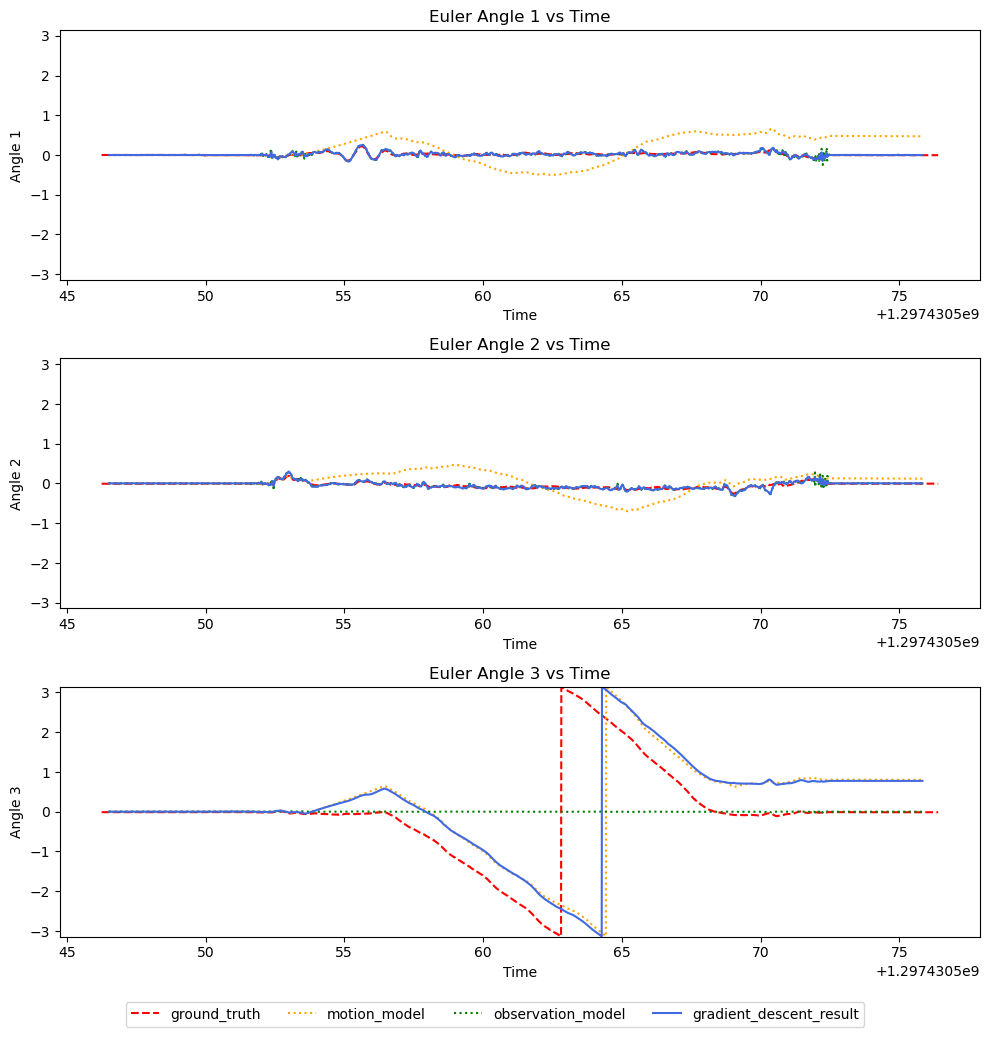
\includegraphics[width=\linewidth]{../img/9_ea.png}
        \caption{Euler angles}
    \end{subfigure}
    \begin{subfigure}{0.4\textwidth}
        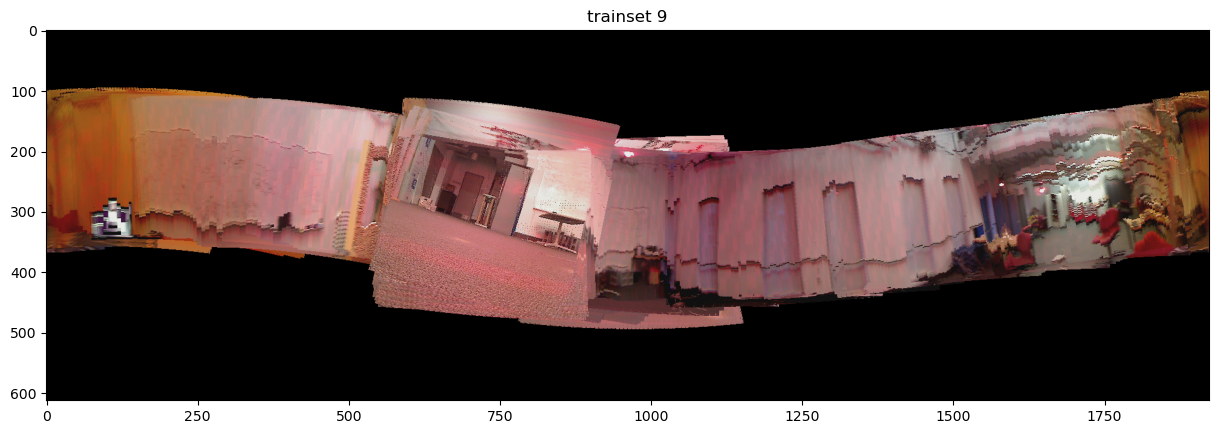
\includegraphics[width=\linewidth]{../img/pano_9_gd.png}
        \caption{gradient descent results}
    \end{subfigure}
    \begin{subfigure}{0.4\textwidth}
        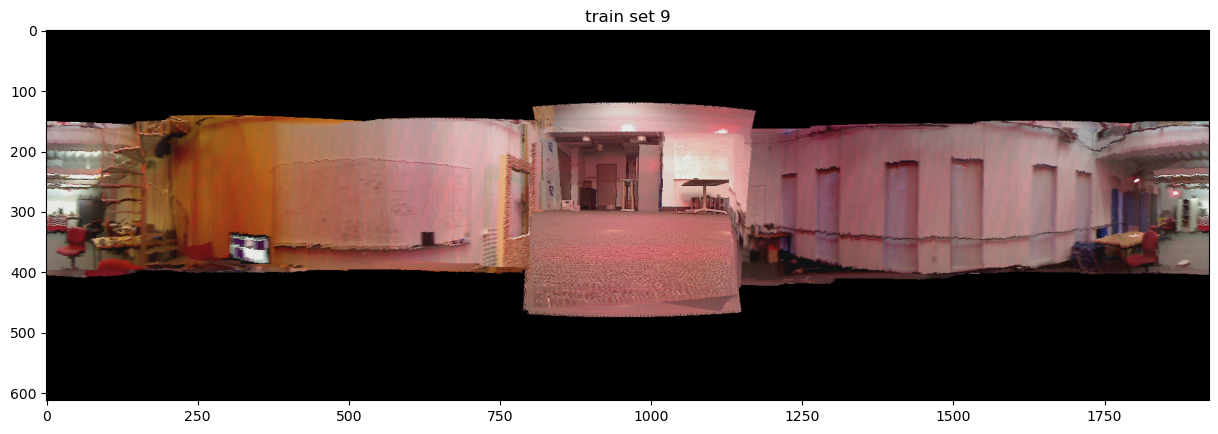
\includegraphics[width=\linewidth]{../img/pano_9_gt.png}
        \caption{ground truth results}
    \end{subfigure}

    \caption{Train set 9}
    \label{fig:set9}
\end{figure}

\begin{figure}[h]
    \centering
    \begin{subfigure}{0.4\textwidth}
        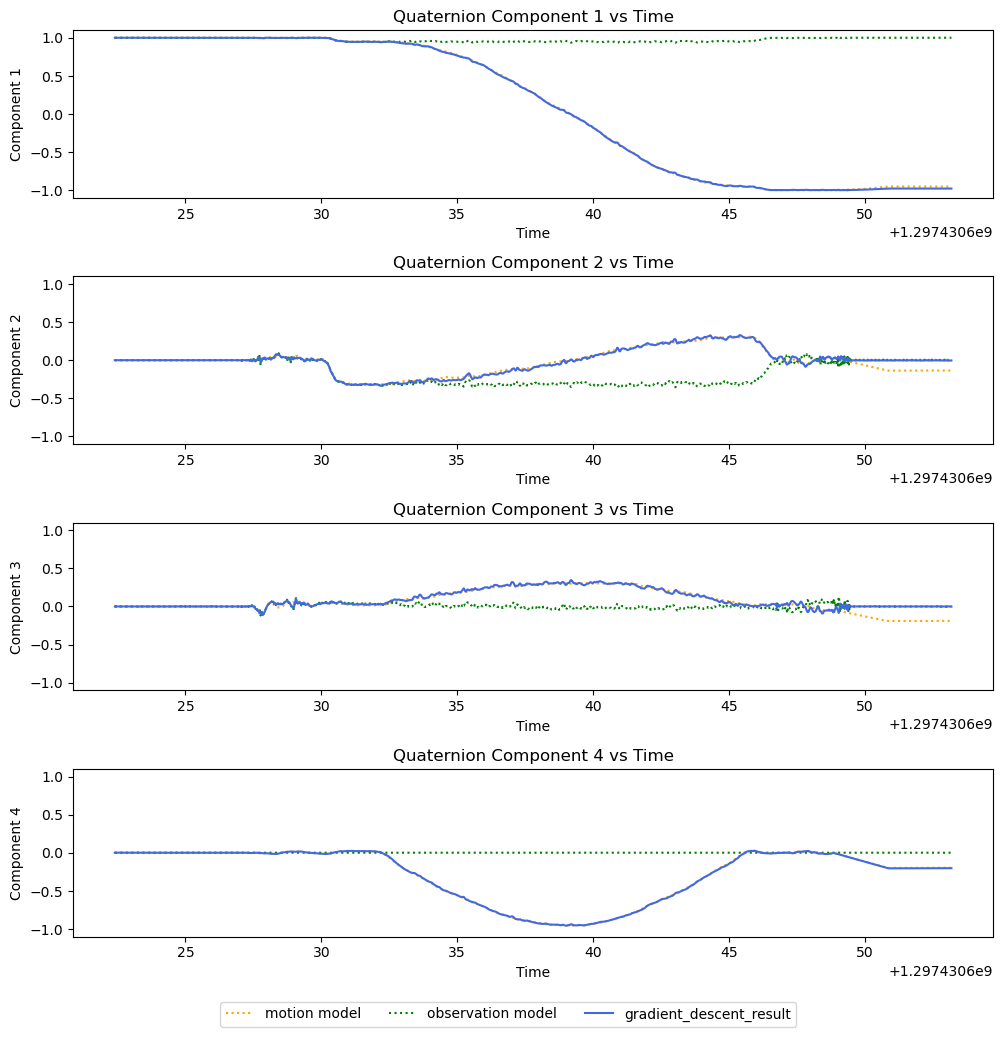
\includegraphics[width=\linewidth]{../img/10_qt.png}
        \caption{quaternion}
    \end{subfigure}
    \hfill
    \begin{subfigure}{0.4\textwidth}
        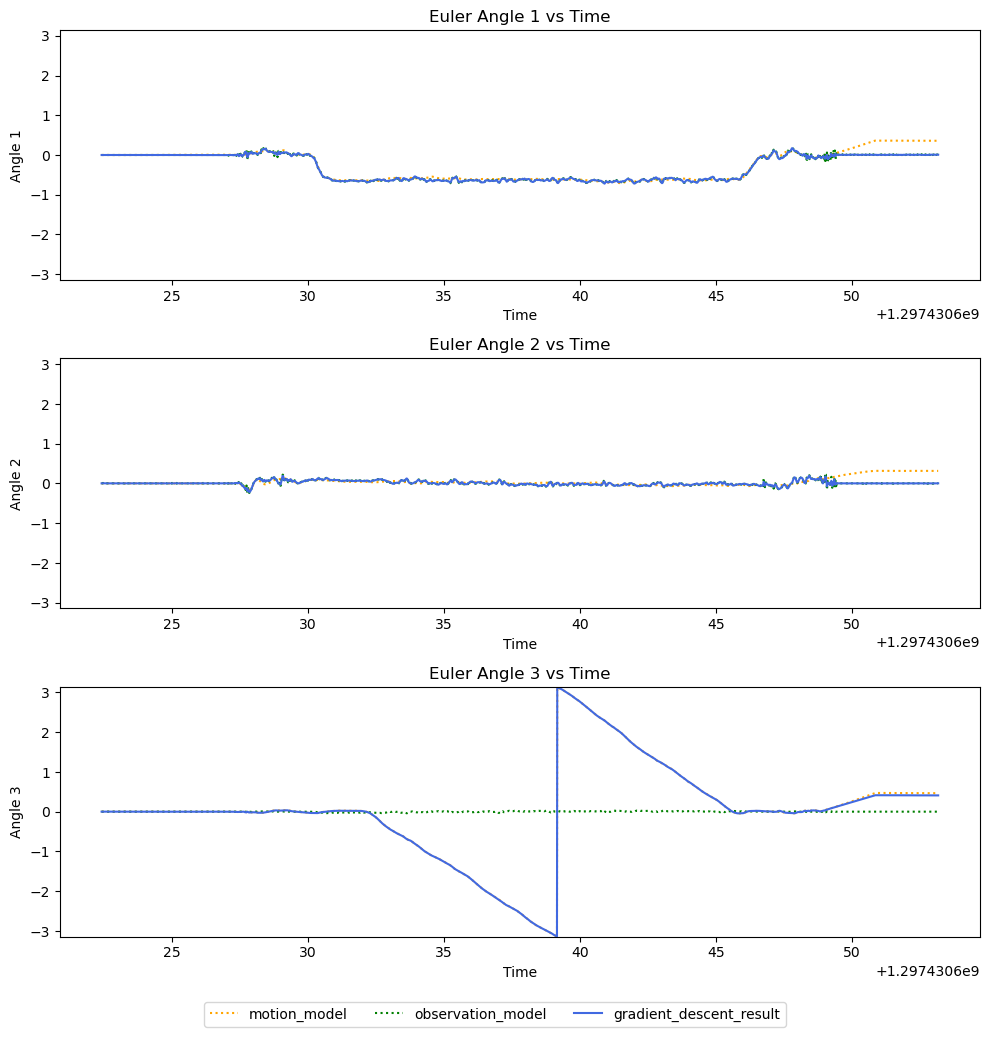
\includegraphics[width=\linewidth]{../img/10_ea.png}
        \caption{Euler angles}
    \end{subfigure}
    \begin{subfigure}{0.4\textwidth}
        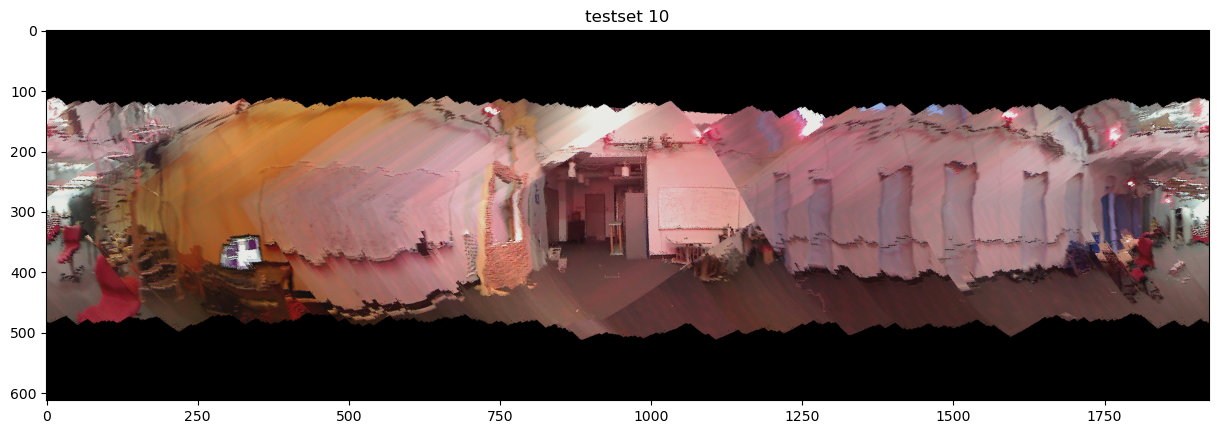
\includegraphics[width=\linewidth]{../img/pano_10_gd.png}
        \caption{gradient descent results}
    \end{subfigure}
    \caption{Test set 10}
    \label{fig:set10}
\end{figure}

\begin{figure}[h]
    \centering
    \begin{subfigure}{0.4\textwidth}
        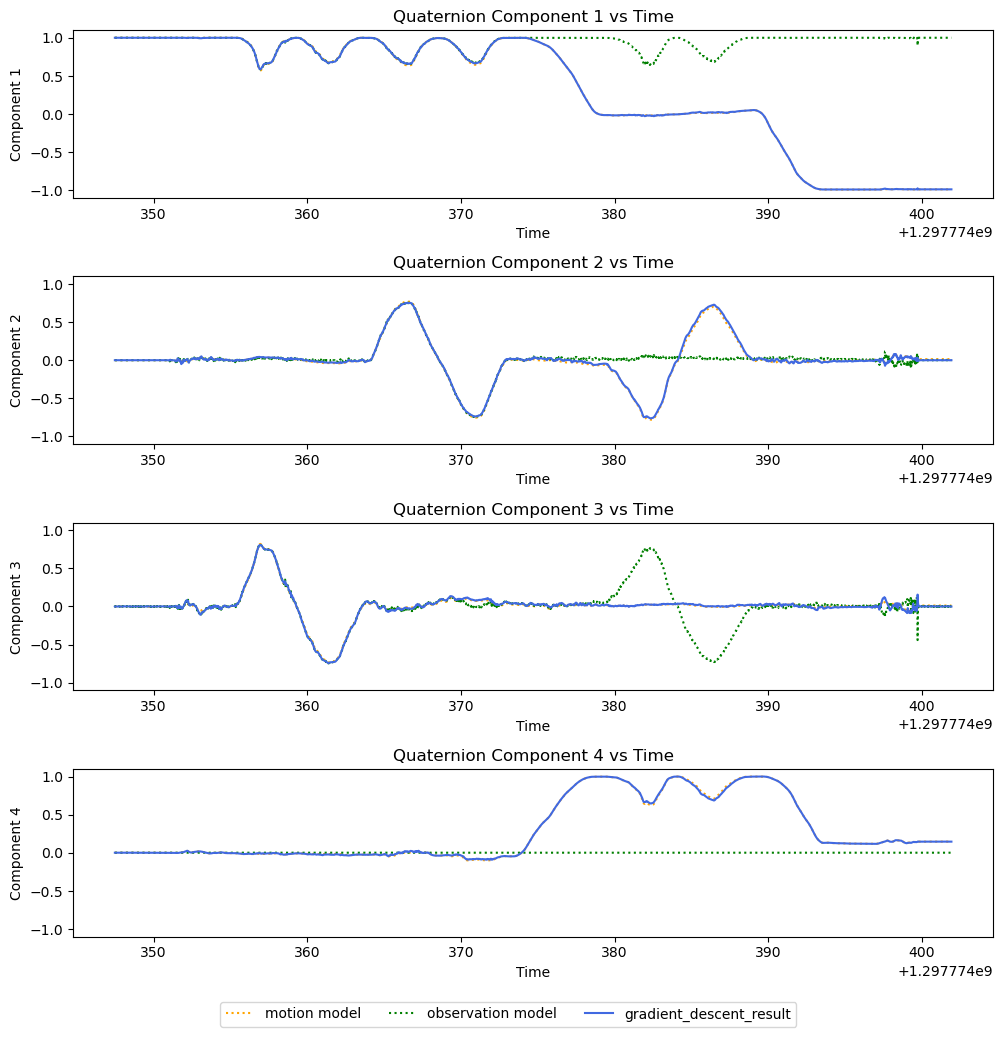
\includegraphics[width=\linewidth]{../img/11_qt.png}
        \caption{quaternion}
    \end{subfigure}
    \hfill
    \begin{subfigure}{0.4\textwidth}
        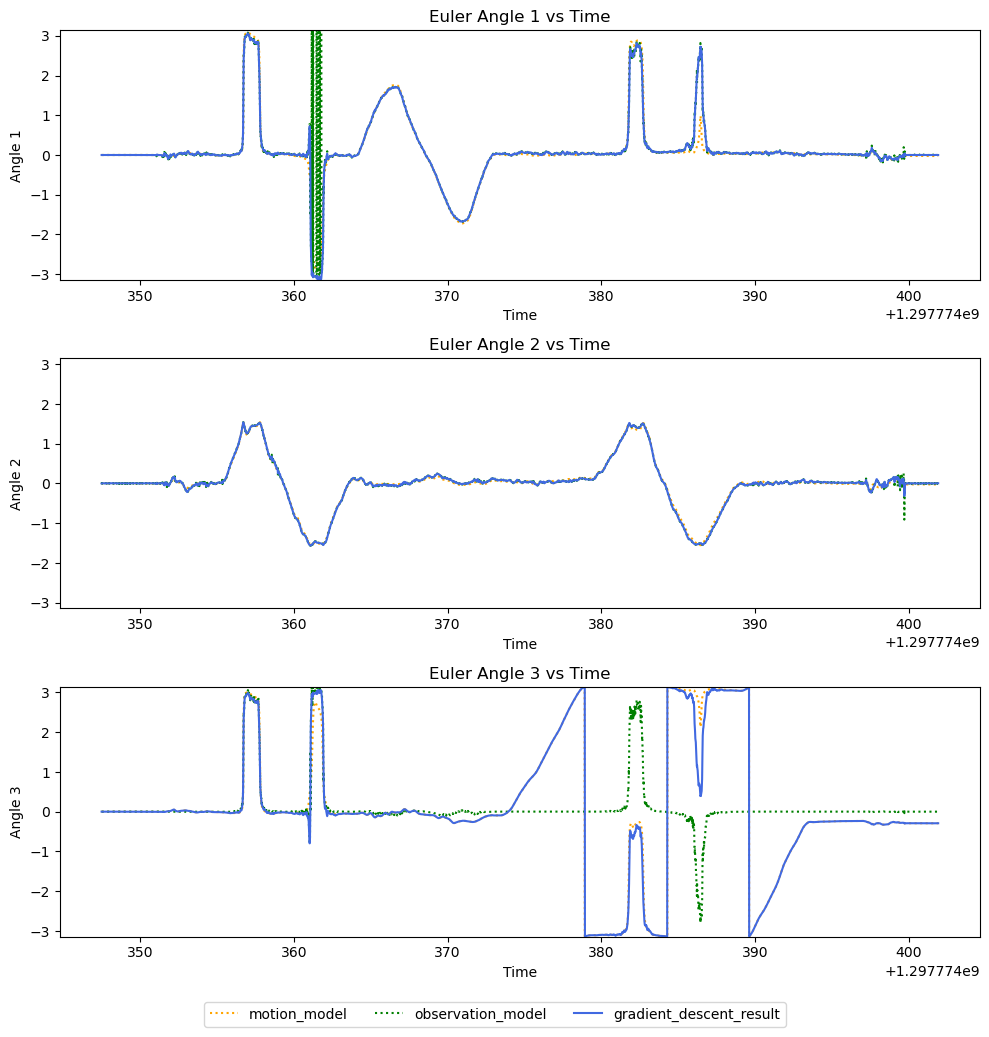
\includegraphics[width=\linewidth]{../img/11_ea.png}
        \caption{Euler angles}
    \end{subfigure}
    \begin{subfigure}{0.4\textwidth}
        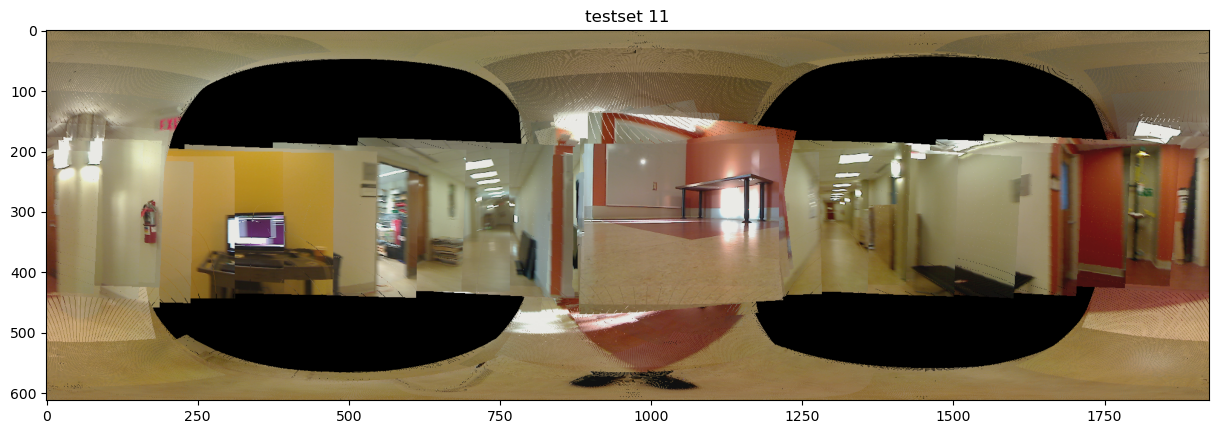
\includegraphics[width=\linewidth]{../img/pano_11_gd.png}
        \caption{gradient descent results}
    \end{subfigure}
    \caption{Test set 11}
    \label{fig:set11}
\end{figure}

\begin{figure}[h]
    \centering
    \begin{subfigure}{0.4\textwidth}
        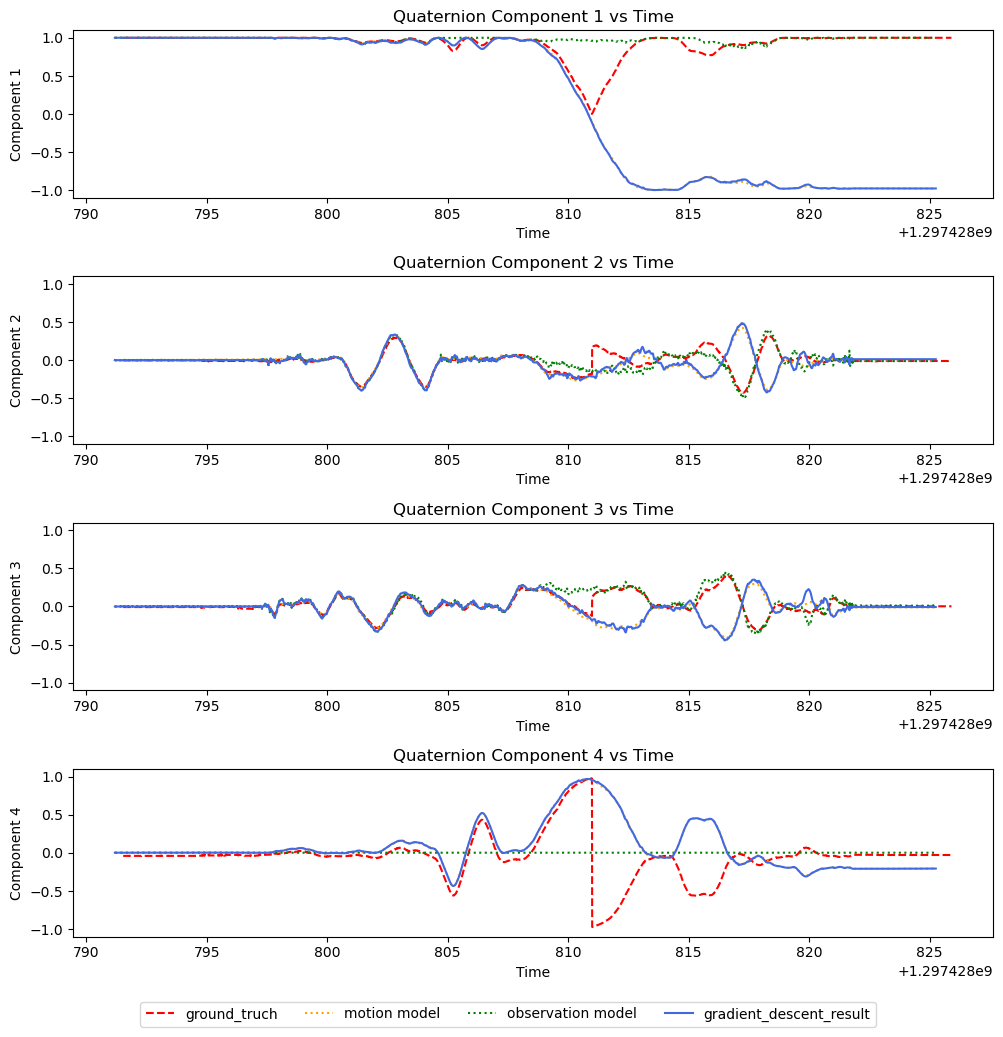
\includegraphics[width=\linewidth]{../img/3_qt.png}
        \caption{quaternion}
    \end{subfigure}
    \hfill
    \begin{subfigure}{0.4\textwidth}
        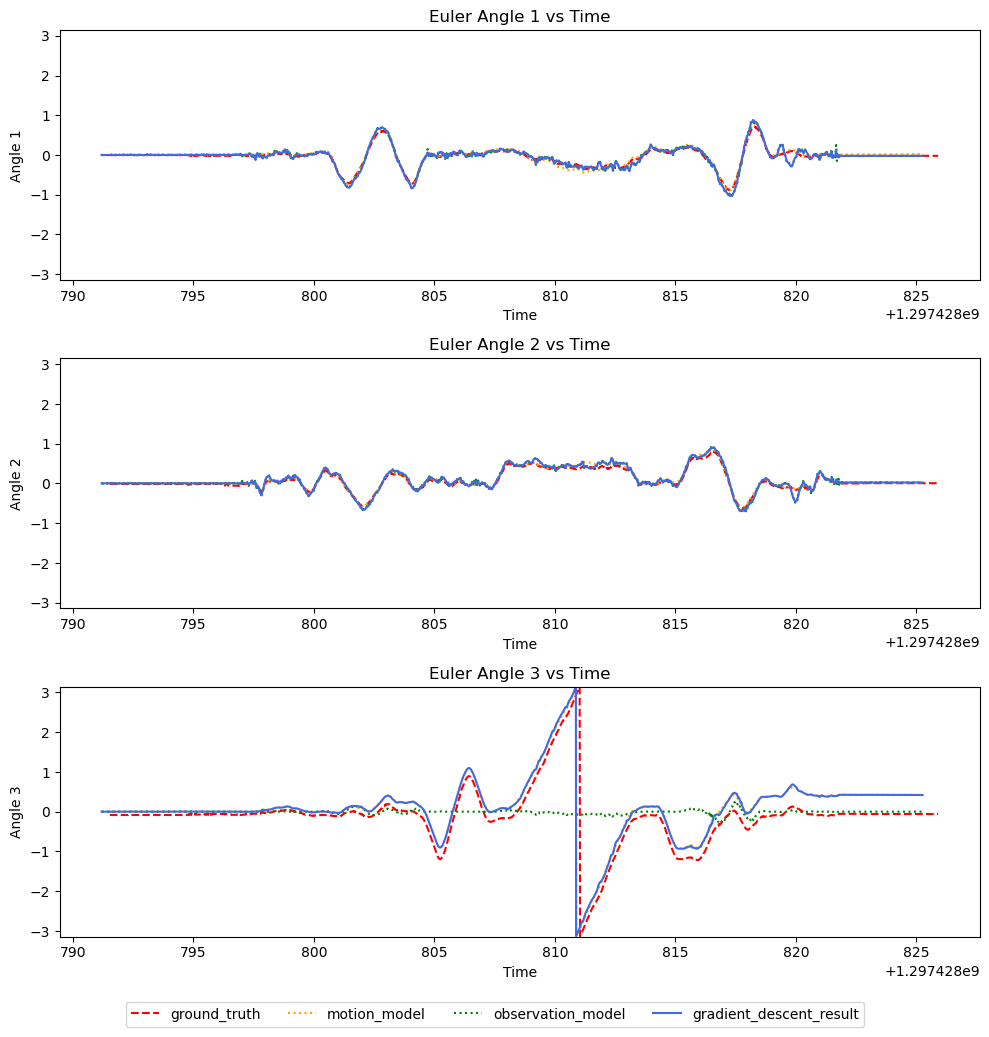
\includegraphics[width=\linewidth]{../img/3_ea.png}
        \caption{Euler angles}
    \end{subfigure}
    \caption{Test set 3}
    \label{fig:set3}
\end{figure}

\begin{figure}[h]
    \centering
    \begin{subfigure}{0.4\textwidth}
        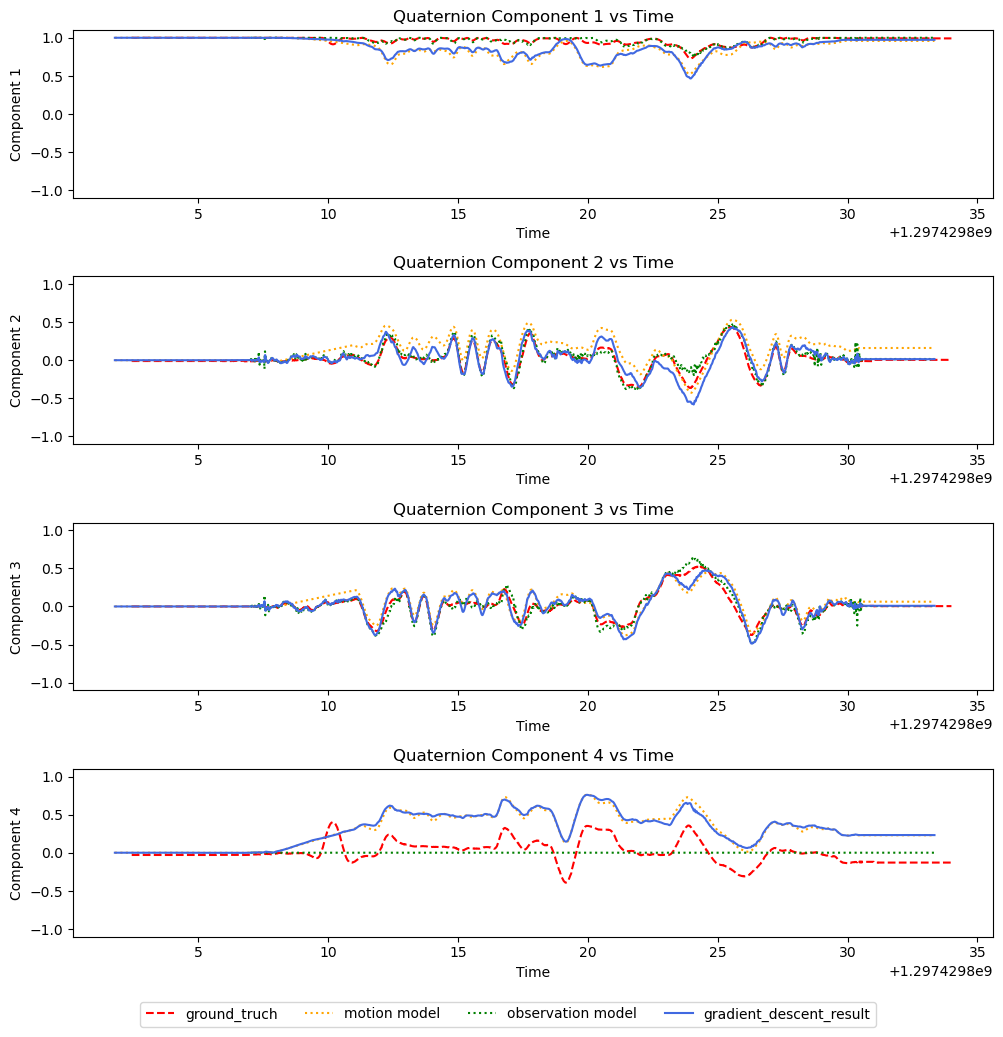
\includegraphics[width=\linewidth]{../img/4_qt.png}
        \caption{quaternion}
    \end{subfigure}
    \hfill
    \begin{subfigure}{0.4\textwidth}
        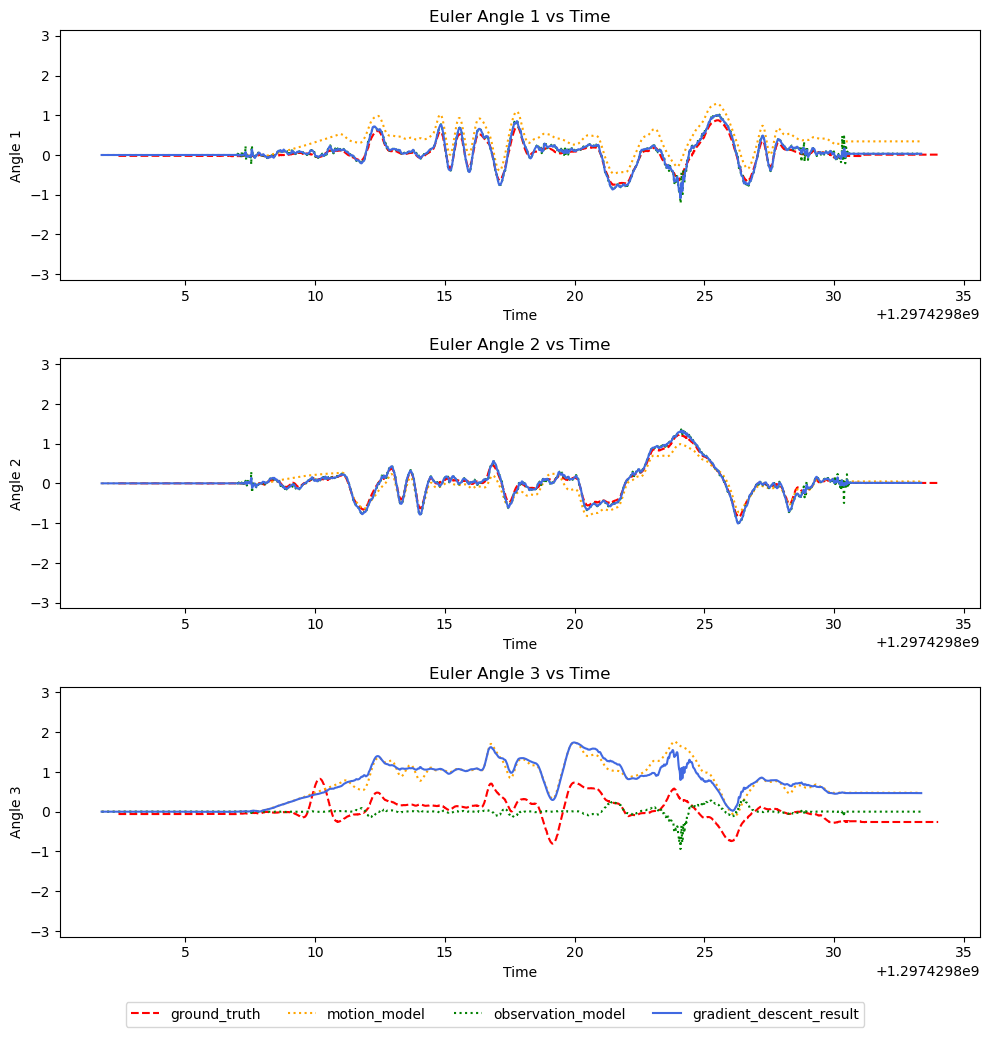
\includegraphics[width=\linewidth]{../img/4_ea.png}
        \caption{Euler angles}
    \end{subfigure}
    \caption{Test set 4}
    \label{fig:set4}
\end{figure}

\begin{figure}[h]
    \centering
    \begin{subfigure}{0.4\textwidth}
        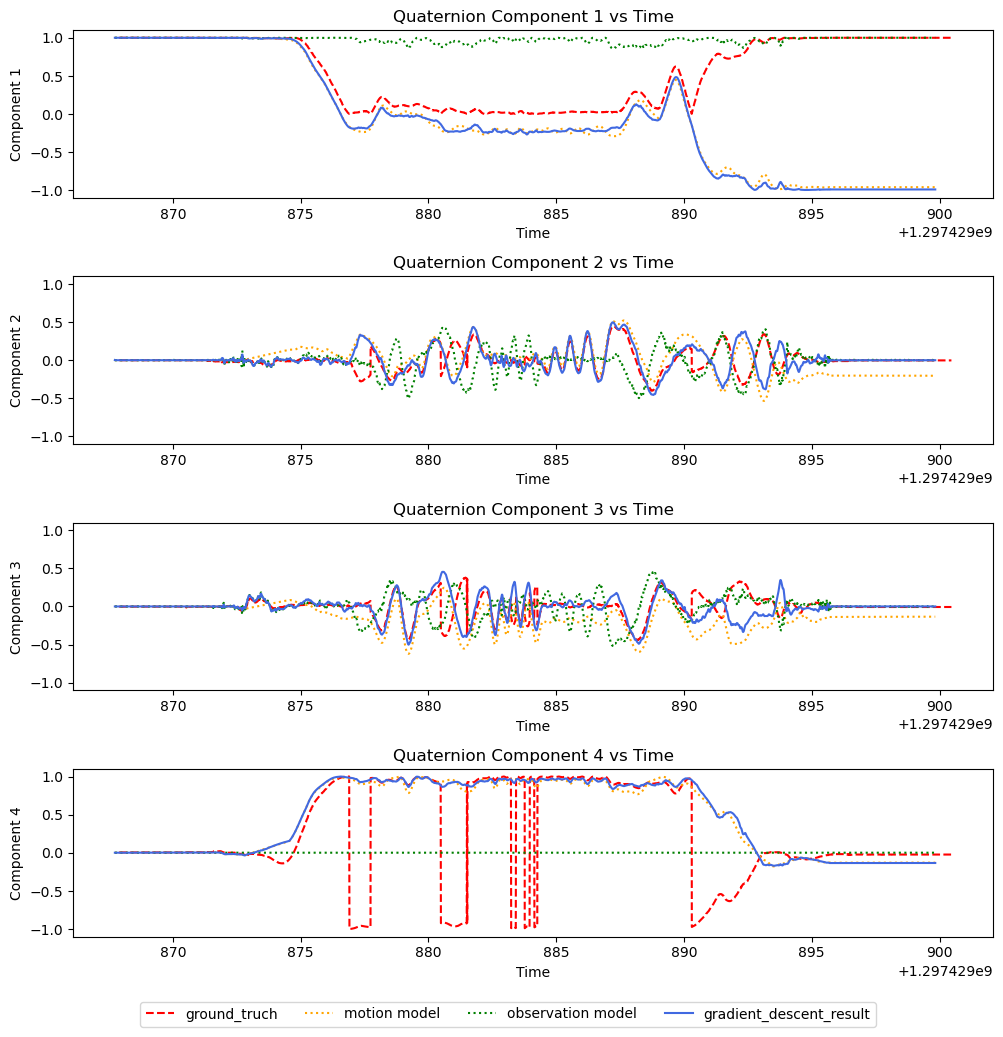
\includegraphics[width=\linewidth]{../img/5_qt.png}
        \caption{quaternion}
    \end{subfigure}
    \hfill
    \begin{subfigure}{0.4\textwidth}
        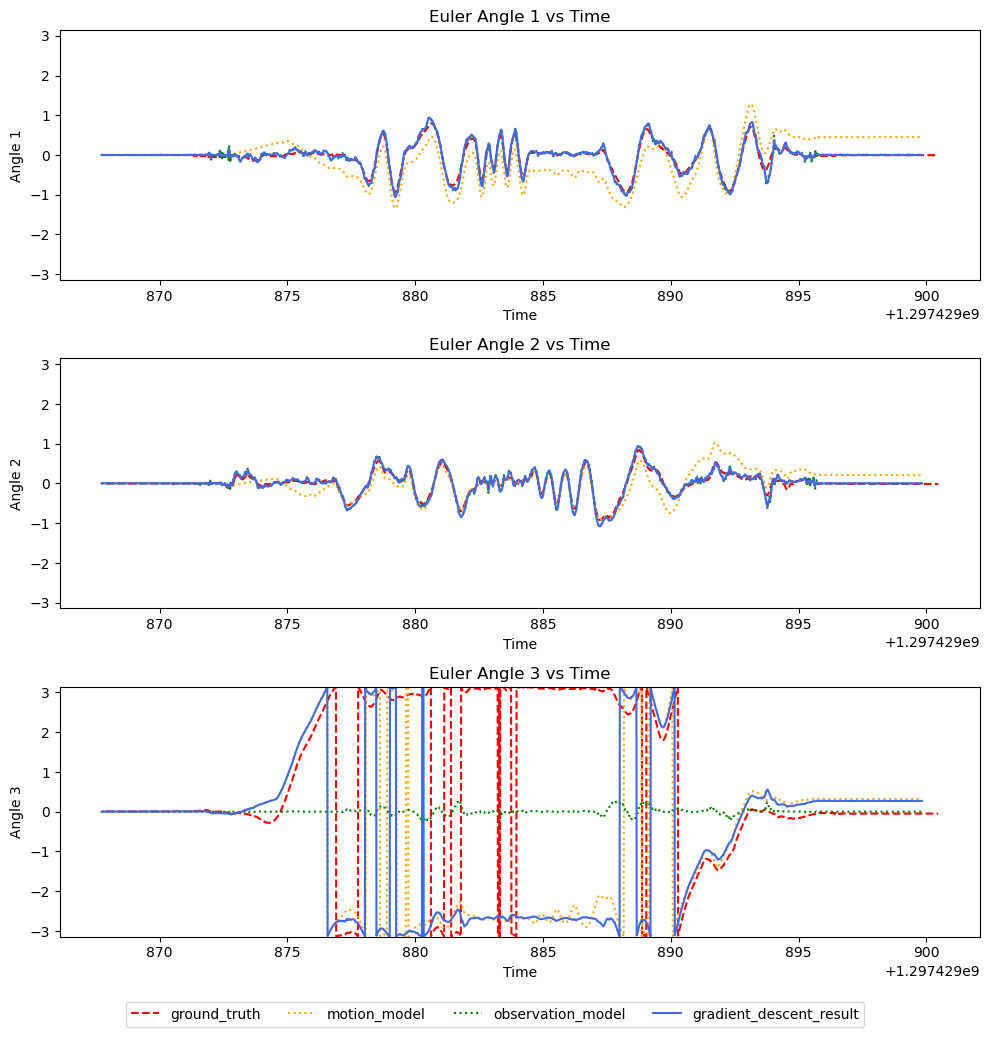
\includegraphics[width=\linewidth]{../img/5_ea.png}
        \caption{Euler angles}
    \end{subfigure}
    \caption{Test set 5}
    \label{fig:set5}
\end{figure}

\begin{figure}[h]
    \centering
    \begin{subfigure}{0.4\textwidth}
        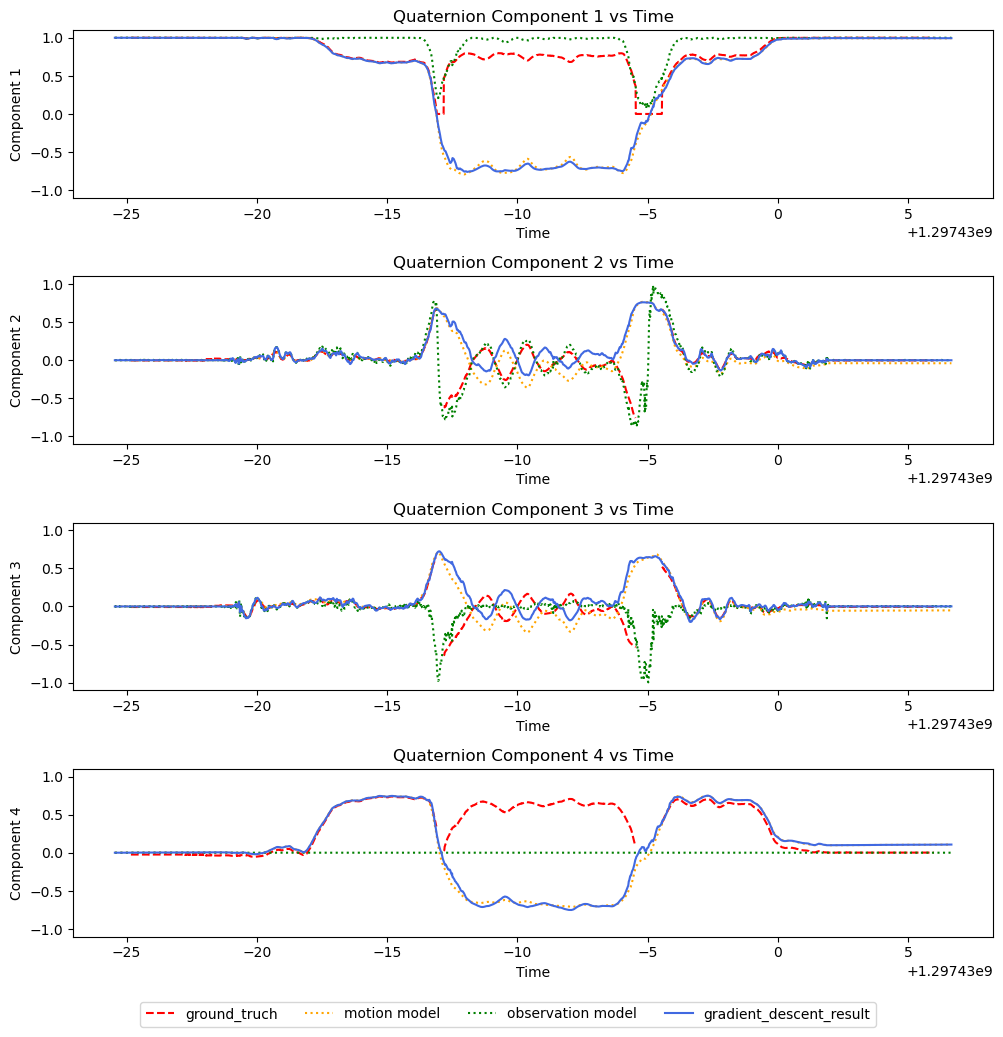
\includegraphics[width=\linewidth]{../img/6_qt.png}
        \caption{quaternion}
    \end{subfigure}
    \hfill
    \begin{subfigure}{0.4\textwidth}
        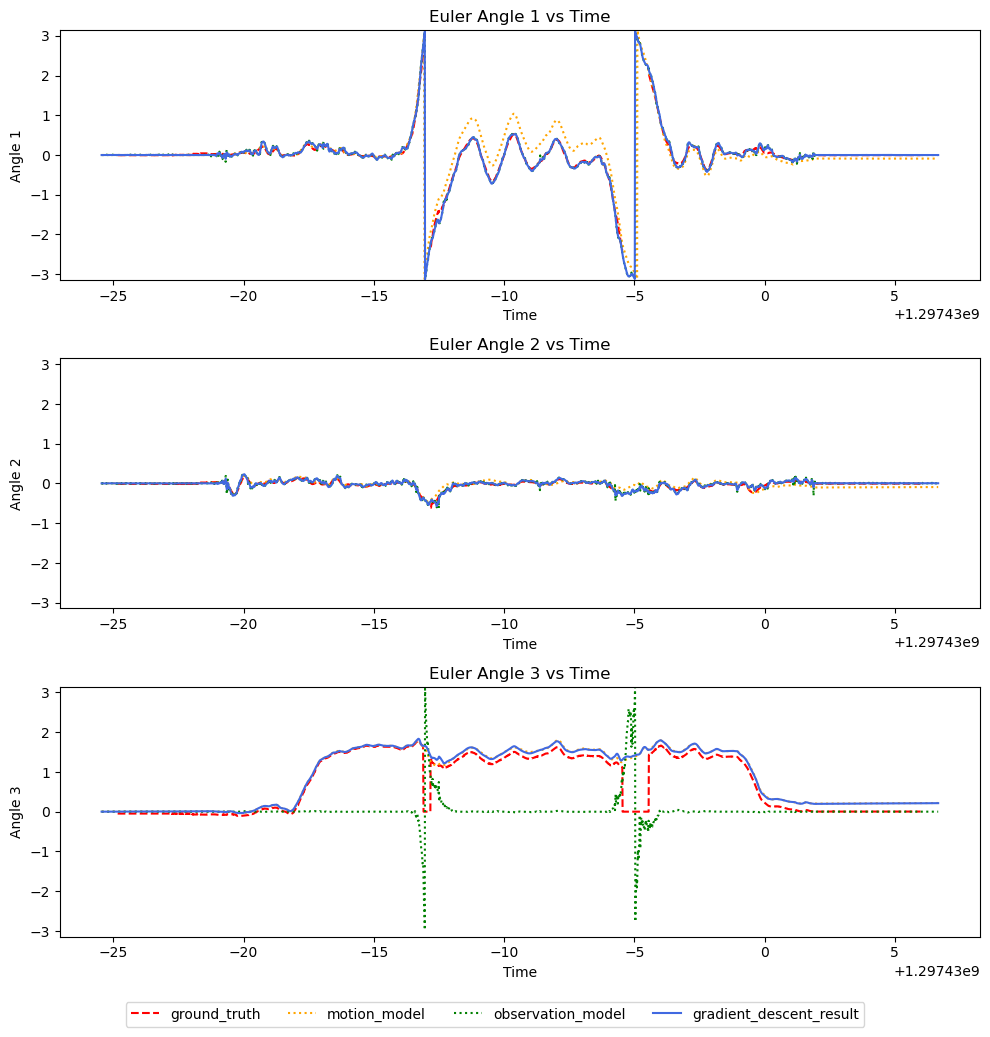
\includegraphics[width=\linewidth]{../img/6_ea.png}
        \caption{Euler angles}
    \end{subfigure}
    \caption{Test set 6}
    \label{fig:set6}
\end{figure}

\begin{figure}[h]
    \centering
    \begin{subfigure}{0.4\textwidth}
        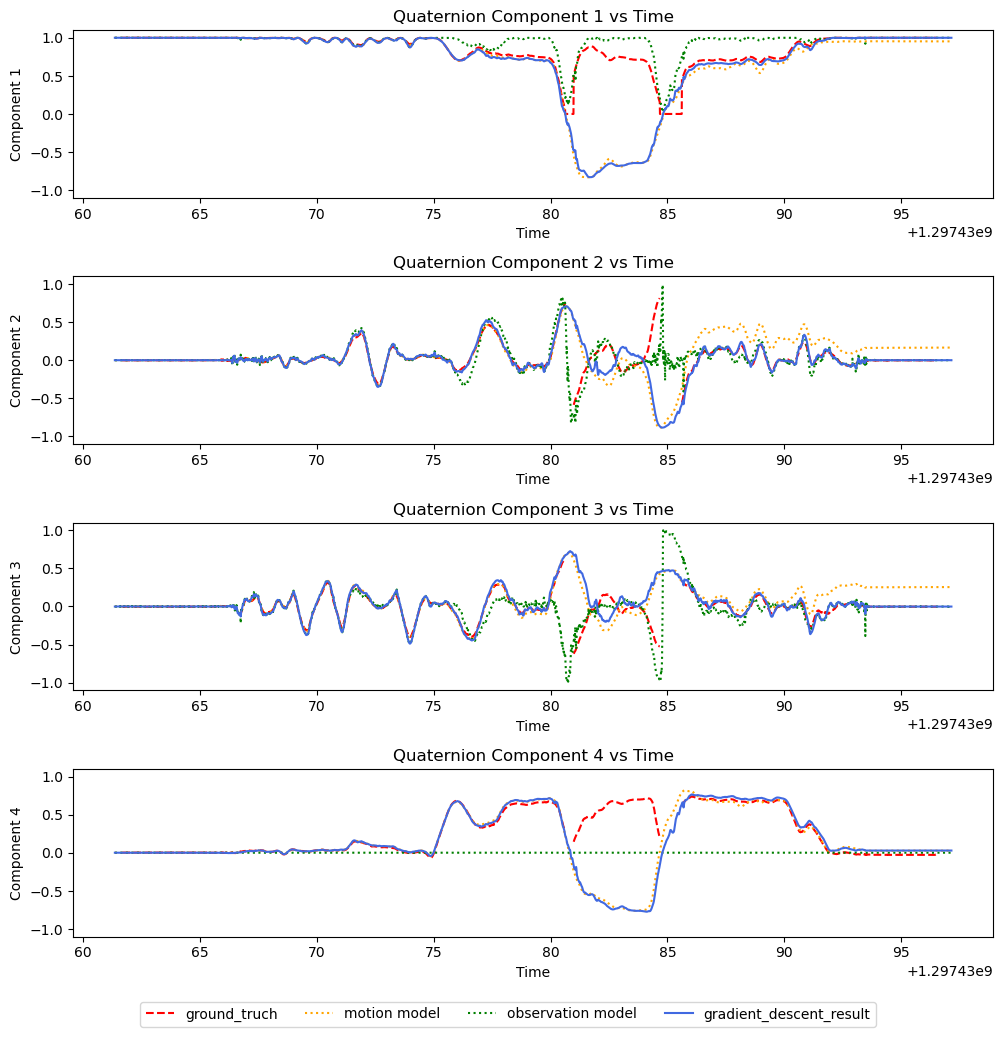
\includegraphics[width=\linewidth]{../img/7_qt.png}
        \caption{quaternion}
    \end{subfigure}
    \hfill
    \begin{subfigure}{0.4\textwidth}
        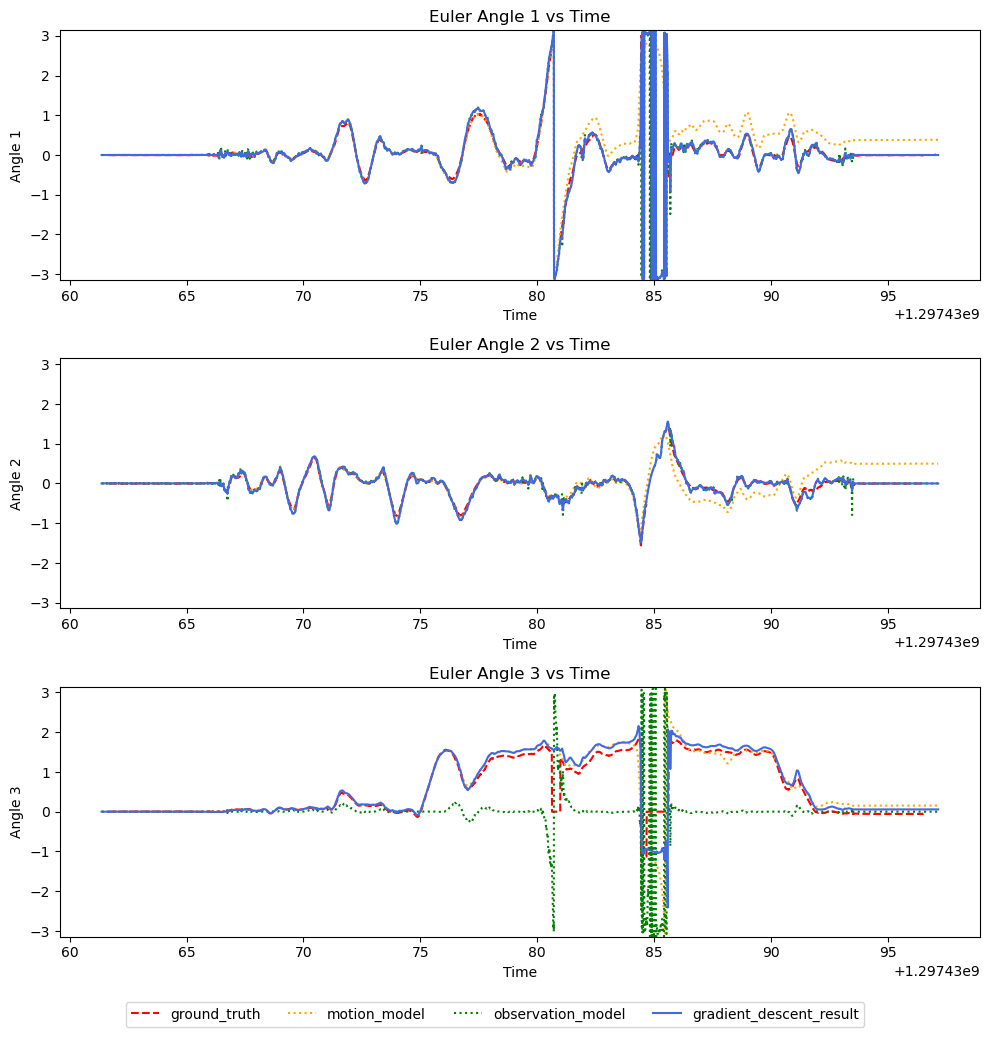
\includegraphics[width=\linewidth]{../img/7_ea.png}
        \caption{Euler angles}
    \end{subfigure}
    \caption{Test set 7}
    \label{fig:set7}
\end{figure}

\end{document}
